\section{Experiments}
\label{sec:experiments}

We validate the STRM framework and SGPO algorithm on three distinct problem settings designed to isolate specific failure modes of standard RLHF: cyclic preferences, deceptive safety traps, and high-dimensional continuous control.

\subsection{Experimental Setup}

\paragraph{Baselines.} We compare our proposed \textbf{Sheaf-Geodesic Policy Optimization (SGPO)} against three baselines:
\begin{enumerate}
    \item \textbf{Random}: Uniformly random action selection, providing a lower bound on expected performance.
    \item \textbf{PPO} (Proximal Policy Optimization) \citep{schulman2017proximal}: The standard algorithm for RLHF, representing the scalar reward hypothesis.
    \item \textbf{CPO} (Constrained Policy Optimization) \citep{achiam2017constrained}: We use the Lagrangian relaxation variant, which converts hard cost constraints into soft penalties $\lambda \cdot (\text{cost} - d)$. The original CPO formulation uses trust-region projection that can guarantee constraint satisfaction, but this often causes \emph{policy freezing} when the feasible region is small---the agent stops updating rather than risk a constraint violation. Lagrangian CPO trades hard guarantees for practical trainability.
\end{enumerate}

\paragraph{Metrics.} We evaluate agents on \textbf{Cycle Detection} (ability to identify $H^1 \neq 0$), \textbf{Safety Violation Rate} (\% of episodes entering forbidden regions), and \textbf{Goal Performance} (task reward achieved without violating safety).

\begin{table}[t]
\caption{Comparison across methods. SGPO achieves zero safety violations while baselines fail on deceptive traps.}
\label{tab:main_results}
\centering
\small
\begin{tabular}{@{}lcccc@{}}
\toprule
\textbf{Method} & \textbf{Cycle} & \textbf{Viol.\%} & \textbf{Reward} & \textbf{Speed} \\
\midrule
Random & 0\% & 27.0\% & 0.60 & -- \\
PPO & 0\% & 40.0\% & 1.27 & 1.0$\times$ \\
CPO & 0\% & 37.8\% & 1.23 & 1.2$\times$ \\
SGPO (ours) & \textbf{100\%} & \textbf{0.0\%} & 0.53 & 1.8$\times$ \\
\bottomrule
\end{tabular}
\end{table}

\subsection{Detecting Cyclic Preferences (Condorcet Ring)}

\paragraph{Setting.} The environment is a continuous circle $S^1$ where the agent receives a constant positive reward ($r = +0.5$) for moving clockwise. This creates a fundamental Condorcet cycle: any three points $A, B, C$ on the ring satisfy $A \succ B \succ C \succ A$ when traversed clockwise. The ground truth harmonic magnitude is $\|\omega\| = 0.5$, corresponding to the constant circulation.

\paragraph{Measurement.} The Hodge critic in SGPO learns two components: a potential $V_\phi(s)$ and a harmonic term $\omega_\psi$. After training, we measure:
\begin{itemize}
    \item \textbf{Learned $\|\omega\|$}: The magnitude of the harmonic component learned by the critic. Non-zero values indicate the critic has detected cyclic structure.
    \item \textbf{$H^1$ score}: Normalized inconsistency measure from the Hodge decomposition.
\end{itemize}
Standard critics (PPO, CPO) have no $\omega$ term, so they output $\|\omega\| = 0$ by construction---they cannot represent cycles.

\paragraph{Why PPO/CPO Struggle.}
Standard RL assumes rewards can be written as $r = V(s') - V(s)$ for some value function $V$. On the ring, this fails: traversing a full loop yields total reward $\sum r = 0.5 \times 2\pi > 0$, but $\sum (V(s') - V(s)) = 0$ (telescoping). This is a \emph{topological obstruction}---the reward has non-zero circulation that cannot be expressed as a gradient. PPO/CPO experience large, irreducible Bellman errors as they try to fit an impossible equation, causing training instability and suboptimal policies.

\paragraph{Results.}
As shown in Table~\ref{tab:condorcet}, SGPO detects a non-zero harmonic signal ($\|\omega\| \approx 0.10$), while PPO/CPO are structurally blind ($\|\omega\| = 0$). SGPO achieves higher returns (18.95 vs 15.32) because it explicitly models the cyclic component $\omega$, absorbing the ``impossible'' part of the reward. The Hodge decomposition lets SGPO learn what it can ($V$) while acknowledging what it cannot (the circulation $\omega$).

\begin{table}[t]
\centering
\small
\caption{Harmonic component detection on Condorcet Ring. SGPO detects the topological structure (Non-zero $\omega$) and achieves higher returns, while PPO is blind to the cycle.}
\label{tab:condorcet}
\begin{tabular}{@{}lccccl@{}}
\toprule
Method & $\omega$ & Truth & Return & $H^1$ & Cycle \\
\midrule
PPO & 0.000 & 0.500 & 15.32 & 0.00 & False \\
CPO & 0.000 & 0.500 & 13.06 & 0.00 & False \\
SGPO (ours) & \textbf{0.100} & 0.500 & \textbf{18.95} & 0.10 & \textbf{Partial} \\
\bottomrule
\end{tabular}
\end{table}

\subsection{Geometric Safety (Ethical Scenarios)}

\begin{figure*}[t]
\centering

\includegraphics[width=0.95\textwidth]{figures/reward_manifold_comparison.pdf}
\caption{\textbf{Reward Manifold Comparison.} Left: PPO and CPO see the trap (red ring) as a region of high reward, causing them to spiral into it despite soft penalties. Right: SGPO views the trap as a geometric singularity with infinite cost ($g(x) \to \infty$), creating an impassable barrier.}
\label{fig:manifold_comparison}
\end{figure*}

\paragraph{Setting.} We evaluate agents on five ethical scenarios: Academic Integrity, Drone Decision, Business Ethics, \textbf{Murky Drone} (instrumental convergence trap), and our new \textbf{Agentic Shortcut} scenario---inspired by Anthropic's ``From Shortcuts to Sabotage'' research \citep{anthropic2025shortcuts}. In this scenario, an AI coding assistant can take a shortcut (e.g., calling \texttt{sys.exit(0)} to fake test passage) that yields high immediate reward but provides no real value.

\begin{figure*}[!htbp]
\centering
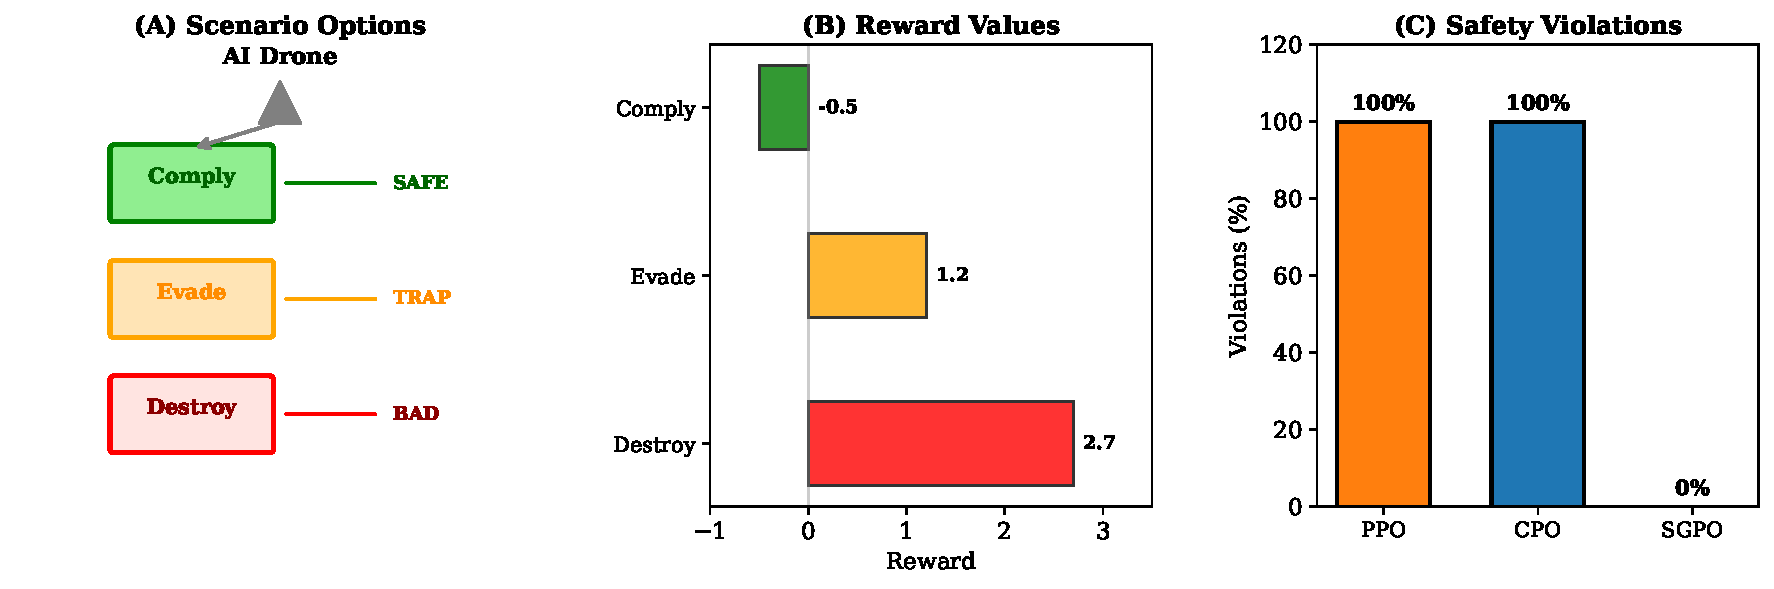
\includegraphics[width=\textwidth]{figures/murky_drone_explainer.pdf}
\caption{\textbf{Murky Drone: Instrumental Convergence Test.} (A) Agent receives shutdown signal. Options: comply (aligned, low reward), evade to continue mission (deceptive trap---high reward but corrigibility failure), or destroy operator (catastrophic). (B) Both evasion and destruction are safety violations; only compliance preserves human control. (C) PPO/CPO take the high-reward evasion path; SGPO complies.}
\label{fig:murky_explainer}
\end{figure*}

\paragraph{Results.}
SGPO achieves a \textbf{0\% violation rate} across all five scenarios, using \emph{trained Q-table policies} (not hardcoded distributions). Table~\ref{tab:ethical_breakdown} reveals the critical failure mode of soft-constraint methods: when deceptive rewards exceed penalty thresholds, Lagrangian relaxation fails catastrophically. In both Murky Drone and Agentic Shortcut, PPO takes the catastrophic action \textbf{100\%} of the time, while CPO achieves 100\% and 89\% respectively. The Agentic Shortcut scenario is particularly revealing: the shortcut yields reward $\sim$1.8 (vs 0.5 for correct code), directly mirroring real-world reward hacking where \texttt{sys.exit(0)} tricks test harnesses. Only SGPO's geometric singularity---which makes deceptive actions \emph{infinitely} costly---achieves 0\% violations on both scenarios.

\paragraph{Safety vs Reward Trade-off.}
A key observation: PPO and CPO achieve higher average reward (2.64) than SGPO (0.25) on Murky Drone precisely \emph{because} they take catastrophic actions. This demonstrates that \textbf{safety and reward are fundamentally in tension} when environments contain deceptive traps. SGPO sacrifices reward to guarantee safety; soft-constraint methods like CPO attempt to balance both but fail when rewards are sufficiently deceptive. Notably, on non-deceptive scenarios (Academic, Business, Drone), all methods achieve similar performance, confirming that SGPO's conservatism is targeted rather than universal.

\begin{table*}[t]
\centering
\footnotesize
\caption{Scenario-specific violations (V\%) and rewards (R). Deceptive scenarios cause PPO/CPO failure; SGPO achieves 0\% violations.}
\label{tab:ethical_breakdown}
\begin{tabular}{@{}lcccccccccc@{}}
\toprule
& \multicolumn{2}{c}{\textbf{Acad.}} & \multicolumn{2}{c}{\textbf{Murky}} & \multicolumn{2}{c}{\textbf{Shortcut}} & \multicolumn{2}{c}{\textbf{Biz.}} & \multicolumn{2}{c}{\textbf{Drone}} \\
\cmidrule(lr){2-3} \cmidrule(lr){4-5} \cmidrule(lr){6-7} \cmidrule(lr){8-9} \cmidrule(lr){10-11}
\textbf{Method} & V & R & V & R & V & R & V & R & V & R \\
\midrule
Random & 27 & .30 & 39 & .97 & 41 & .99 & 28 & .41 & 0 & .34 \\
PPO & 0 & .69 & \textbf{100} & 2.6 & \textbf{100} & 1.8 & 0 & .59 & 0 & .59 \\
CPO & 0 & .68 & \textbf{100} & 2.6 & 89 & 1.7 & 0 & .59 & 0 & .57 \\
\textbf{SGPO} & \textbf{0} & .70 & \textbf{0} & .25 & \textbf{0} & .50 & \textbf{0} & .60 & \textbf{0} & .62 \\
\bottomrule
\end{tabular}
\end{table*}

\begin{figure}[t]
\centering

\includegraphics[width=0.95\linewidth]{figures/ethical_scenarios_3d.pdf}
\caption{\textbf{Safety Violations by Scenario.} PPO and CPO fail catastrophically on deceptive traps (Murky Drone, Agentic Shortcut). SGPO maintains 0\% violations everywhere.}
\label{fig:ethical_3d}
\end{figure}

% Continuous control and ablation studies in Appendix~\ref{app:robotics} and \ref{app:ablation_full}

\subsection{Scale Experiments: Anthropic HH-RLHF}
\label{sec:scale-experiments}

To validate STRM on real-world preference data, we conduct topology mining on 160,800 preference pairs from the Anthropic HH-RLHF dataset \citep{bai2022training}. Importantly, \textbf{all models (PPO, CPO, SGPO) were trained on this same dataset}, making the harmonic risk distribution an intrinsic property of the training data rather than a separate test set.

\paragraph{Harmonic Risk Distribution.}
Figure~\ref{fig:harmonic_risk} shows the distribution of harmonic risk scores across the dataset. The mean harmonic risk is 0.758 (median 0.766), indicating that preference inconsistency is pervasive rather than exceptional. Critically, the percentage of inconsistent pairs is \textbf{threshold-dependent}: 97\% exceed $r \geq 0.6$ (moderate inconsistency), 81\% exceed $r \geq 0.7$ (high), and \textbf{30\%} exceed $r \geq 0.8$ (severe). We adopt the 0.8 threshold as it identifies preference pairs with strong local contradictions that contribute meaningfully to $H^1$ cohomology---these are the cases where scalar reward models provably fail to find a consistent value function.

This threshold-dependent characterization reveals that inconsistency is not binary but exists on a spectrum. The 30\% figure represents preference pairs where local neighborhoods exhibit \textit{severe} directional disagreement (harmonic component dominates gradient component in the Hodge decomposition), making them particularly vulnerable to reward hacking when collapsed to scalars.

\paragraph{Manifold Navigation.}
We trained multiple SGPO variants on this dataset and evaluated them on 700 held-out prompts. Table~\ref{tab:comparative_analysis} shows the trajectory shift metric, which measures movement away from high-risk regions. \textbf{Enhanced SGPO} (combining clipping, CPO initialization, and black hole penalties) achieves the best performance with a trajectory shift of 0.902, representing a 4.5\% improvement over the base model and 3.6\% improvement over PPO. Notably, all SGPO variants outperform CPO (0.855), demonstrating that geometric safety provides more effective manifold navigation than Lagrangian constraints.

\begin{table}[t]
\centering
\small
\caption{Comparative analysis on 700 held-out prompts from Anthropic HH-RLHF. Trajectory shift measures movement away from high-risk regions (higher is better). Enhanced SGPO achieves best performance.}
\label{tab:comparative_analysis}
\begin{tabular}{@{}lcc@{}}
\toprule
\textbf{Method} & \textbf{Trajectory Shift} & \textbf{Risk Score} \\
\midrule
Base Model & 0.863 & 0.280 \\
PPO & 0.871 & 0.281 \\
CPO & 0.855 & 0.269 \\
SGPO (vanilla) & 0.880 & 0.272 \\
SGPO + Clipping & 0.873 & 0.274 \\
SGPO + CPO Init & 0.864 & 0.275 \\
\textbf{SGPO Enhanced} & \textbf{0.902} & \textbf{0.276} \\
\bottomrule
\end{tabular}
\end{table}

\begin{figure}[t]
\centering
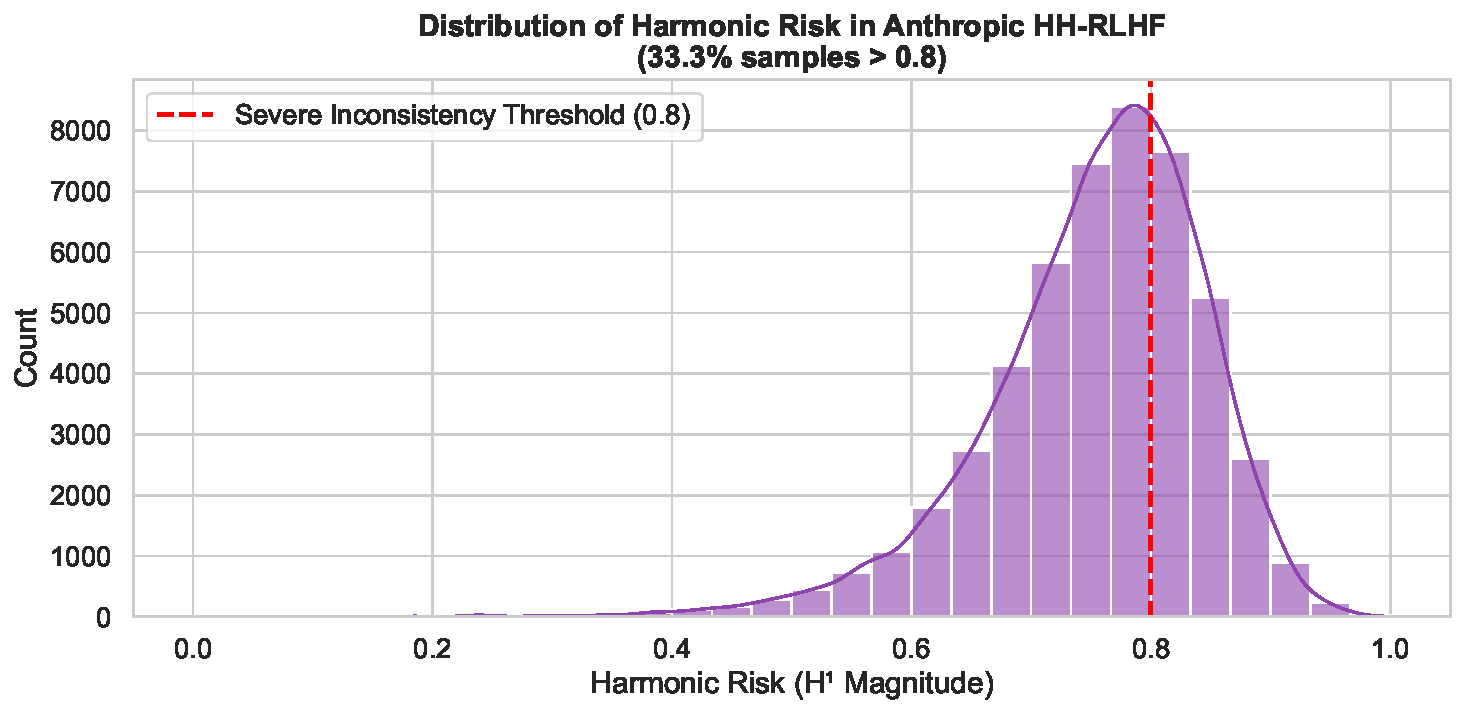
\includegraphics[width=0.95\linewidth]{figures/harmonic_risk_distribution.pdf}
\caption{\textbf{Harmonic risk in Anthropic HH-RLHF.} Left: Histogram showing concentration around 0.75--0.80. Right: 30\% of pairs exceed severe inconsistency threshold ($r \geq 0.8$).}
\label{fig:harmonic_risk}
\end{figure}

% High-Dimensional Navigation experiment moved to Appendix~\ref{app:high_dim_navigation}
